\setcounter{chapter}{2}
\chapter{Capítulo III: \\Marco Metodológico}
\thispagestyle{empty}

\section{Hipótesis de Trabajo }
Como sugiere Huertas en su escrito La Formulación de la Hipótesis \cite{huertas} las hipótesis se materializan luego que el investigador llega a través de la observación a una proposición inicial. La observación nos lleva a una creencia común del mercado bursátil de Colombia de que la TRM esta correlacionada al precio del barril de petróleo. Al llevar esta proposición al análisis, se nota que la correlación es real pero no completa. Hay otros elementos adicionales al precio internacional de petróleo que forman parte de un modelo predictivo, y que quizás compartan la similitud de ser variables relacionadas con los productos de mayor exportación y contribuyentes a la agregación del producto bruto interno.

La pregunta de investigación entonces evoluciona a la siguientes:

\emph{¿Como crear un modelo predictivo de la TRM de Colombia usando Aprendizaje Automatizado basándonos en los productos de mayor contribución a la canasta del producto bruto interno?}

El elemento de aprendizaje automatizado es una condición de la solución innovadora solo por un hecho. Como nos explica Prabanjhan \cite{narayanachar}): “el aprendizaje automatizado utiliza datos estadísticos y métodos estadísticos y de computación avanzados para aprender de un juego y muestras de datos y entrenar un modelo con validación cruzada… “. A diferencia de las metodologías estadísticas anteriores donde el investigador utiliza los estudios y análisis de los datos para crear un modelo, el aprendizaje automatizado toma los datos y nos permite entrenar los datos para resolver el problema del modelo. Como los datos entrenados se validan de forma cruzada con el modelo, el modelo subsiguiente ya tiene su propio error estadístico implícitamente delimitado, lo que nos permite utilizarlo con un grado de confianza medible desde el punto de vista matemático.

Utilizando técnicas de investigación exploratoria visual es evidente que solo la variable descriptora del precio internacional de petróleo no es suficiente, sino que hay otros factores que influyen en el precio de la TRM y que la mantienen de subir mucho y los efectos nefastos de la devaluación que esto acarrea. De aquí entonces nuestra hipótesis general de trabajo:

\emph{El valor de la TRM se puede pronosticar a través de un modelo estadístico parsimonioso basado en los datos históricos de la valorización de los productos de mayor contribución al portafolio de exportaciones de Colombia.}

\subsection{Hipótesis especificas}
Las siguientes son hipótesis específicas de trabajo.

\begin{itemize}
	\item Existen una cantidad finita - e inferior a la decena - de productos de exportación que fungen como variables de agregación al producto bruto interno de Colombia y que son necesarias para la consecución de un modelo predictivo parsimonioso de la TRM.
	\item El valor de la TRM, tal cual lo ja la Superintendencia Financiera de Colombia, no es sino el reflejo de los movimientos de estas variables de aportación que ayudan a modelar y controlar la tasa de cambio.
	\item El comportamiento pasado de dichas variables puede ser utilizado para entrenar y generar un modelo estadístico predictivo parsimonioso utilizando aprendizaje automatizado cuyo margen de error sea inferior al 5\% (o, en otros términos, \(p < 0.05\)).
	\item El modelo final no es único sino es el resultado del ensamblaje de varios modelos matemáticos predictivos y dinámico en su concepción ya que puede ser afectado por la acumulación de nuevos datos de retroalimentación a posteriori (N. Del A. esta hipótesis es especulativa en naturaleza, y experimentación matemática precisa es necesaria para validarla).
\end{itemize}

\section{Metodología de Estudio}
Enfoque cuantitativo experimental utilizando Machine Learning.

\begin{itemize}
	\item Método ensamblado de GLM y ARIMA
	\item Aprendizaje automatizado
	\item Biblioteca CARET para la creación de muestras aleatorias de entrenamiento y evaluación cruzada
	\item 70\% datos de entrenamiento
	\item 30\% datos de evaluación cruzada
\end{itemize}

\section{Descripción del Método}
La metodología utilizada para el trabajo de investigación se apega estrictamente a la formalización de la hipótesis de trabajo:

\begin{equation}
    p^{c}(x) = (p^{c}(c_{1} \mid x),p^{c}(c_{2} \mid x))
\end{equation}

Donde:

\begin{eqnarray}
    c_{1} & : & y_{t}^{\prime} = c + \phi_{1}y_{t-1}^{\prime} + \ldots + \phi_{p}y_{t-p}^{\prime} + \phi_{1}e_{t-1} + \ldots + \phi_{q}e_{t-q} + e_{t} \\
    c_{2} & : & f(y_{t}) = \beta_{0} + \beta_{1}x_{t-1} + \beta_{2}x_{t-2} + \cdots + \beta_{n}x_{t-n} + \epsilon_{t}
\end{eqnarray}

Por lo tanto la metodología del estudio se puede resumir en un método ensamblado de aprendizaje automatizado resultante de la composición de dos aprendices: uno basado en un regresor lineal y el segundo basado en un pronostico ARIMA. Los valores estimados para cada caso del arreglo de datos se utilizan como variable independiente y predictor del modelo ensamblado, con la variable dependiente inmutable. El modelo ensamblado entonces se entrena nuevamente con los resultados de las predicciones contra los valores reales \cite{leek}.

Podemos resumir el proceso con el siguiente esquema de arquitectura del modelo:

\begin{figure}[h!]
    \centering
    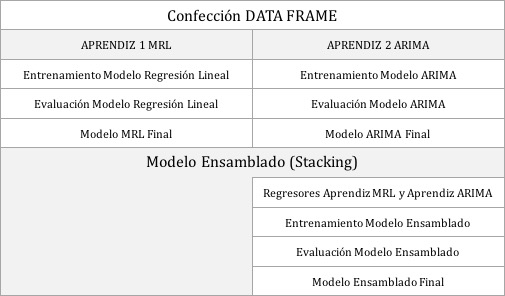
\includegraphics[width=5in]{ArquitecturaModeloEnsamblado}
    \caption{Proceso de Investigación para el Análisis del Modelo Predictivo (Fuente Propia)}
\end{figure}

Cada aprendiz es a su vez un modelo de aprendizaje automatizado con su propia metodología de investigación.

\subsubsection{Aprendiz 1: Modelo de Regresión Lineal}
\begin{itemize}
	\item El aprendiz 1 es un modelo de regresión lineal utilizando como variable dependiente el valor de la TRM para cada día del juego de datos y como regresores un arreglo asociado de cotizaciones del precio promedio mundial de los once productos principales de la canasta de exportación de Colombia entre los años 2010 y 2017.
	\item Para el juego de entrenamiento se selecciona un 70\% de los datos disponibles. Dicha selección se hace con la ayuda de la biblioteca CARET de R para funciones de aprendizaje automatizado.
	\item Para el juego de validación se selecciona un 30\% de los datos disponibles. Dicha selección también se hace con la ayuda de la biblioteca CARET de R para funciones de aprendizaje automatizado.
	\item La variable SEED se prefigura al valor arbitrario \emph{7556014} para propósitos de reproducibilidad de los datos.
	\item El aprendizaje automatizado no asegura que todos los regresores sean útiles o necesarios para una predicción dentro de los valores de confianza esperados. Existe la posibilidad que un número limitado de regresores cumpla con los mismos valores de predicción que la totalidad de los mismos y que el modelo generalice mejor al tener menos regresores (disminuyendo la inflación de la varianza como efecto secundario).
	\item Para determinar el número óptimo de regresores se procedió a armar el modelo de aprendizaje automatizado sumando un regresor a la vez y analizando los valores del coeficiente de determinación y coeficiente de correlación. Los valores finales del error mínimo cuadrático de cada modelo se comparan para determinar la mejor combinación de regresores.
	\item Como segunda validación para la combinación correcta de regresores, se utilizó el análisis \emph{Step\_AIC} (reducción óptima de regresores utilizando análisis combinatorio y el Criterio de Información de Aikake) con la biblioteca \emph{STEP\_AIC} de \emph{R}. El método \emph{STEP\_AIC} es intensivo en recursos de computación y no siempre arroja resultados superiores a los que un investigador pueda armar a mano utilizando técnicas visuales de exploración de datos.
\end{itemize}

\subsubsection{Aprendiz 2: Modelo ARIMA}
\begin{itemize}
	\item El aprendiz 2 es un modelo de pronostico ARIMA utilizando como serie de tiempo el valor de la TRM para cada día del juego de datos entre los años 2010 y 2017.
	\item Para el juego de entrenamiento se selecciona un 70\% de los datos disponibles. Dicha selección se hace con la ayuda de la biblioteca FORECAST de R para funciones de aprendizaje automatizado utilizando series de tiempo \cite{hyndman}.
	\item Para el juego de validación se selecciona un 30\% de los datos disponibles. Dicha selección también se hace con la ayuda de la biblioteca FORECAST de R para funciones de aprendizaje automatizado de series de tiempo.
	\item La variable SEED se prefigura al valor arbitrario \emph{7556014} para propósitos de reproducibilidad de los datos.
\end{itemize}

\subsubsection{Clasificador Ensamblado}
\begin{itemize}
	\item El clasificador ensamblado se toma como un arreglo de una variable dependiente (el valor de la TRM para cada día correspondiente al juego de datos) y dos variables independientes (los resultados de la predicción de los dos aprendices).
	\item Para el juego de entrenamiento se selecciona el 100\% de los datos disponibles. Dicha selección se hace con los resultados de las pruebas de evaluación de los dos aprendices iniciales \cite{popularEnsemble}.
	\item La variable SEED se prefigura al valor arbitrario \emph{7556014} para propósitos de reproducibilidad de los datos.
	\item El modelo se resuelve utilizando la metodología de Stacking como un modelo de regresión lineal \cite{smolyakov}.
\end{itemize}

\subsubsection{Validación del Modelo Ensamblado}
Se espera del modelo final un nivel de desempeño con predicciones dentro de un \(\alpha \leq 0.05\). Para tal fin dentro del diseño de investigación se valida el modelo sometiendo el mismo a un juego aleatorio de 100 datos de muestra que comprende:

\subsubsection{Esquema Visual del Modelo Predictivo}
El siguiente es el esquema visual del modelo predictivo donde se muestra como los resultados de los aprendices del modelo ARIMA y de regresión lineal múltiple se convierten en las entradas del modelo ensamblado.

\begin{figure}[H]
	\centering
	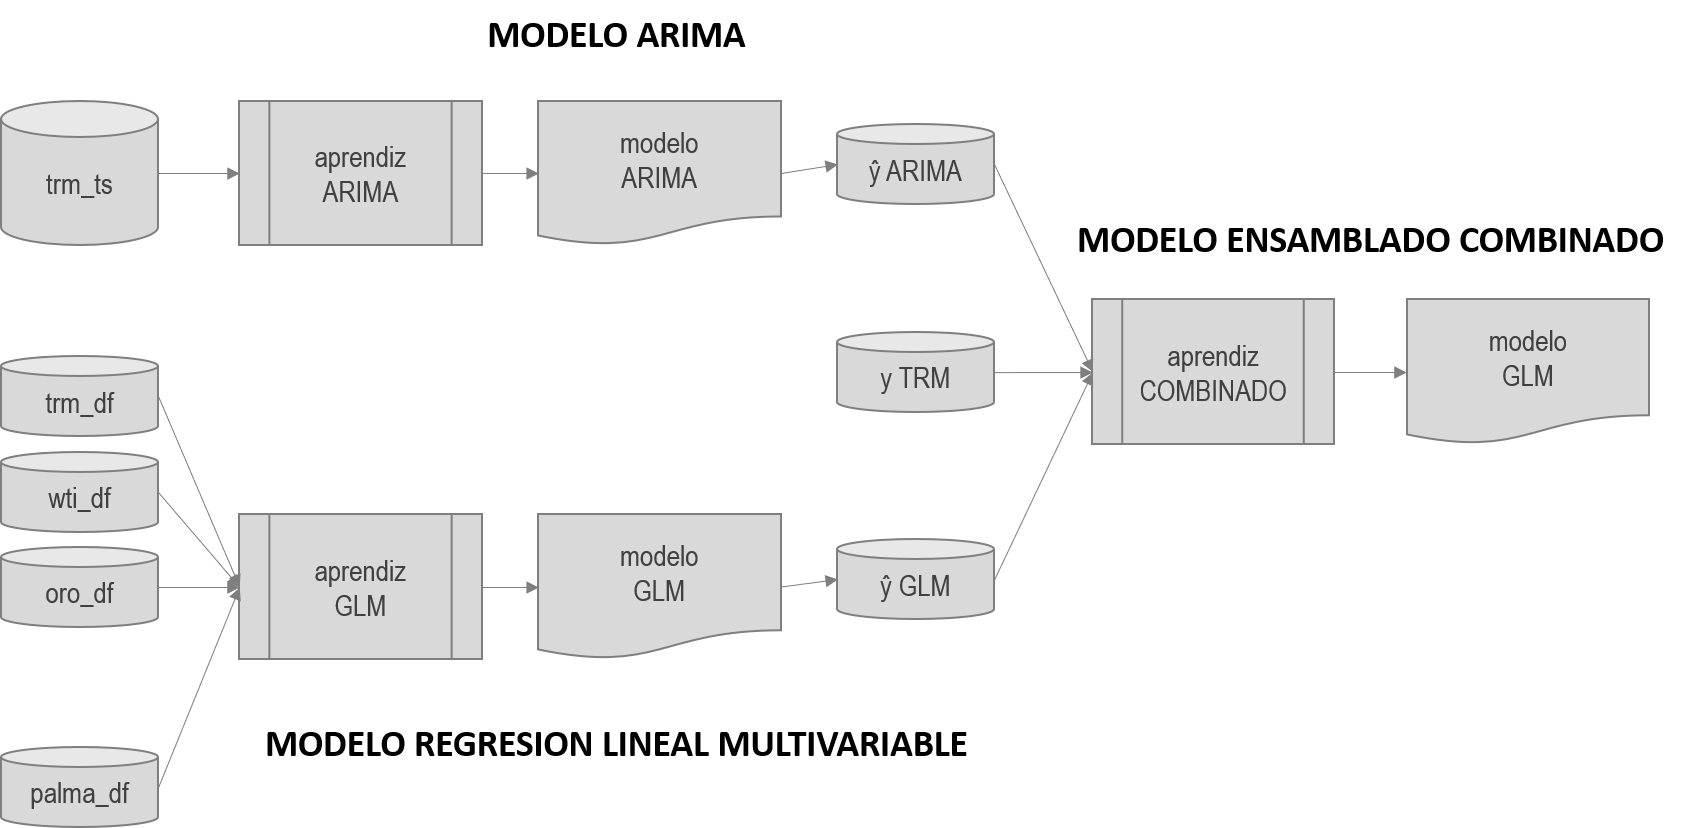
\includegraphics[width=5in]{images/EsquemaModeloPredictivo.png}	\caption{Esquema Modelo Predictivo}
\end{figure}

\begin{itemize}
	\item Resultados de predicción del modelo versus el modelo aprendiz 1 de regresión lineal multivariable.
	\item Resultados de predicción del modelo ensamblado versus el modelo aprendiz 2 ARIMA.
	\item Resultados de predicción del modelo ensamblado versus un intervalo de confianza del 99\%.
\end{itemize}

El modelo se considera óptimo para producción si pasa las tres pruebas de validación.

\section{Diseño de la Instrumentación}
El diseño de la instrumentación para el trabajo de laboratorio incluirá programas de software matemático para:

\begin{itemize}
    \item Recolectar las diferentes series de tiempo que servirán como variables dependientes (valor de la TRM) e independientes (regresores tales como las cotizaciones del barril de petróleo, quintal de café, etc.)
    \item Análisis exploratorio visual para determinar validez de los datos, muestras de autocorrelación y autocorrelación parcial a través de la prueba Dickey-Fueller
    \item Calce de la función de regresión lineal para las variables independientes
    \item Código para el modelo predictivo ensamblado
\end{itemize}

\subsection{Componentes de Investigación Series de Tiempo}
Un componente de aportación es cualquier rubro que se supone se exporta desde Colombia, aporta ingresos en dólares, y por lo tanto ayuda a equilibrar la balanza de pagos y demanda demanda de divisas - y por ende la TRM. Es importante hacer un análisis de cada uno de estos que debe incluir \cite{zumelMount}:

\begin{itemize}
	\item carga inicial como serie de tiempo (time series class)
	\item start(), end()
    \item summary()
    \item plot.ts()
    \item acf()
    \item pacf()
    \item descomponer en stl()
    \item prueba Dickey Fuller adf.test()
\end{itemize}

La carga inicial de datos para cualquier serie de tiempo se hace a través del servicio web de \textit{Quandl} (el siguiente ejemplo ilustrativo utiliza las cotizaciones del quintal de café).

\begin{lstlisting}[language=R]
# Load coffee prices as time series
library(Quandl)
library(tseries)

Quandl.api_key("KzzS8Vfxkw1ZgTWgU4jH")
coffee <- Quandl("ODA/PCOFFOTM_USD", collapse = "monthly", type = "ts")
head(coffee)
class(coffee)
cycle(coffee)
\end{lstlisting}

\subsection{EDA (Explorative Data Analysis)}
La forma más sencilla de ver los efectos del precio del café es revisar la tendencia del precio internacional y si ha habido efectos por temporada o alguna tendencia \cite{daroczi}.

\begin{lstlisting}[language=R]
plot.ts(coffee)
abline(reg = lm(coffee ~ time(coffee)))
\end{lstlisting}

\begin{figure}[H]
	\centering
	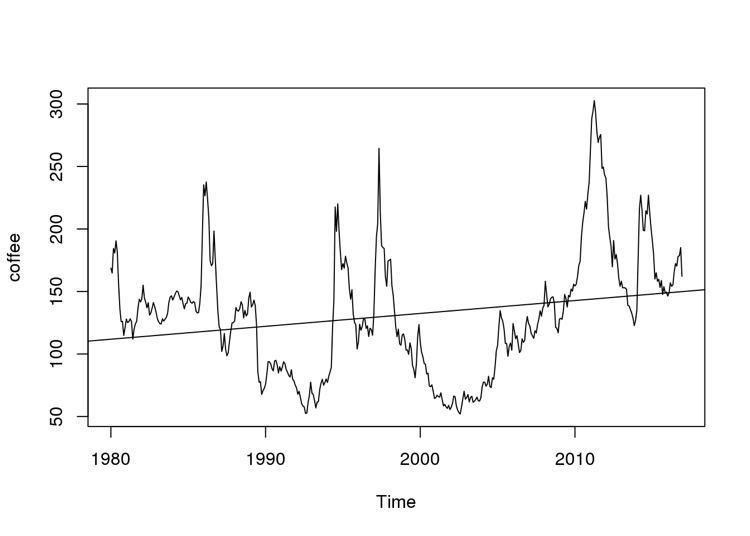
\includegraphics[width=5in]{correlacionTiempoCafe}
	\caption{Análisis EDA Cotización Internacional Café por quintal  (Fuente Propia)}
\end{figure}

Otro examen necesario es el de autocorrelación y autocorrelación parcial. Ambos análisis nos permiten ver si la serie es del tipo auto-regresiva o de promedios móviles \cite{hyndman}.

\begin{lstlisting}[language=R]
par(mfrow=c(1,2))
acf(coffee)
pacf(coffee)
\end{lstlisting}

\begin{figure}[H]
	\centering
	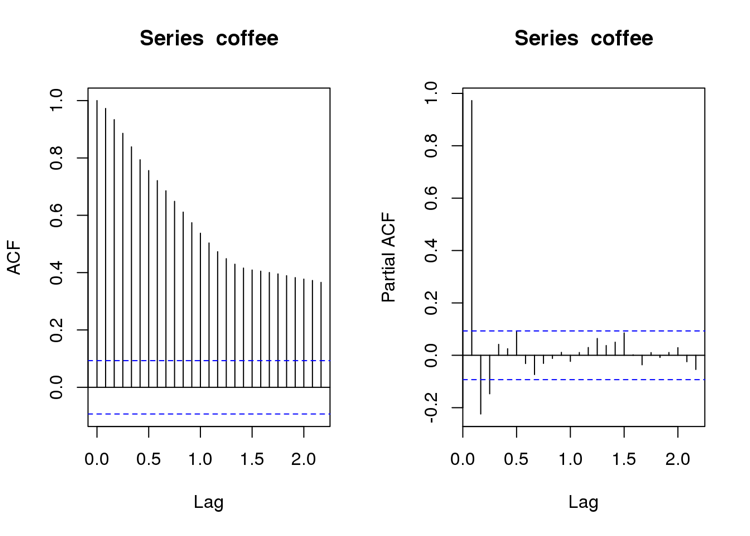
\includegraphics[width=5in]{autocorrelacion}\\
	\caption{Correlograma Precio Internacional del Café (Fuente Propia)}
\end{figure}

El último examen es la descomposición de la serie en datos, temporalidad y tendencia, para ver si alguno de estos elementos está presente.

\begin{lstlisting}[language=R]
decomp <- stl(coffee, s.window = 11)
plot(decomp)
\end{lstlisting}

\begin{figure}[H]
	\centering
	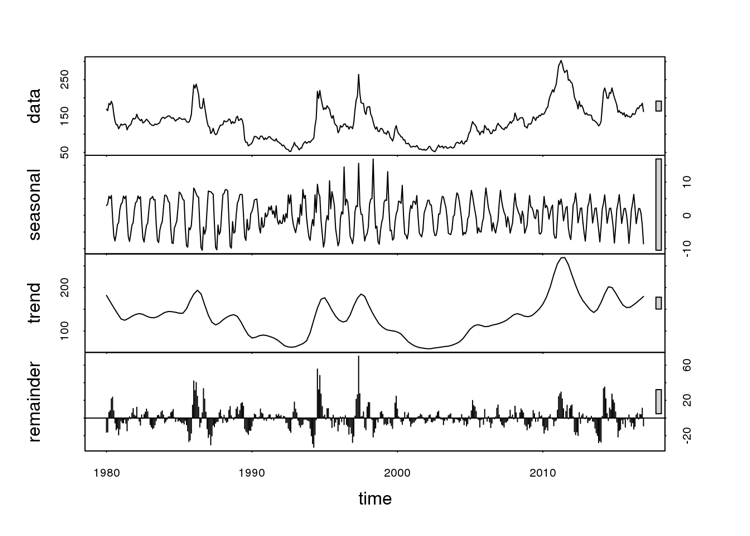
\includegraphics[width=5in]{decopSTLCafe}\\
	\caption{Descomposición STL Precio Internacional del Café (Fuente Propia)}
\end{figure}

El test \emph{Dickey Fuller} \cite{dickeyfuller} es la prueba mas importante para la verificación de la estacionalidad de una serie de tiempos. La literatura recomienda altamente someter todas las pruebas de series al test \emph{Dickey Fuller} antes de proceder con otros análisis \cite{hyndman}.

\begin{lstlisting}[language=R]
# Dickey Fuller Test for stationary time series
df <- adf.test(coffee, k = 12)
df$statistic
df$p.value
\end{lstlisting}

\subsection{Regresión Lineal con Calce de la Función de Predicción}
Los modelos de regresión lineal utilizan la biblioteca \emph{Quandl} para la extracción de datos y deben hacer la transformación del arreglo de datos a una serie de tiempos. Los datos serán colapsados de forma mensual y se revisará la fórmula de la función de calce para el coeficiente de correlación y determinación \cite{narayanachar}.

\begin{lstlisting}[language=R]
# Load oil prices as time series
library(Quandl)
library(tseries)

Quandl.api_key("KzzS8Vfxkw1ZgTWgU4jH")
wti <- Quandl("EIA/PET_RWTC_D", collapse = "monthly", type = "ts")
head(wti)
class(wti)
cycle(wti)

plot.ts(wti)
abline(reg = lm(wti ~ time(wti)), col="red")
fit = lm(wti ~ time(wti))
summary(fit)


Call:
lm(formula = wti ~ time(wti))

Residuals:
    Min      1Q  Median      3Q     Max
-45.031 -13.929  -0.368  11.399  80.925

Coefficients:
              Estimate Std. Error t value Pr(>|t|)
(Intercept) -4849.3862   213.2634  -22.74   <2e-16 ***
time(wti)       2.4439     0.1065   22.94   <2e-16 ***
---
Signif. codes:  0 '***' 0.001 '**' 0.01 '*' 0.05 '.' 0.1 ' ' 1

Residual standard error: 19.43 on 384 degrees of freedom
Multiple R-squared:  0.5782,	Adjusted R-squared:  0.5771
F-statistic: 526.4 on 1 and 384 DF,  p-value: < 2.2e-16
\end{lstlisting}

\begin{figure}[H]
	\centering
	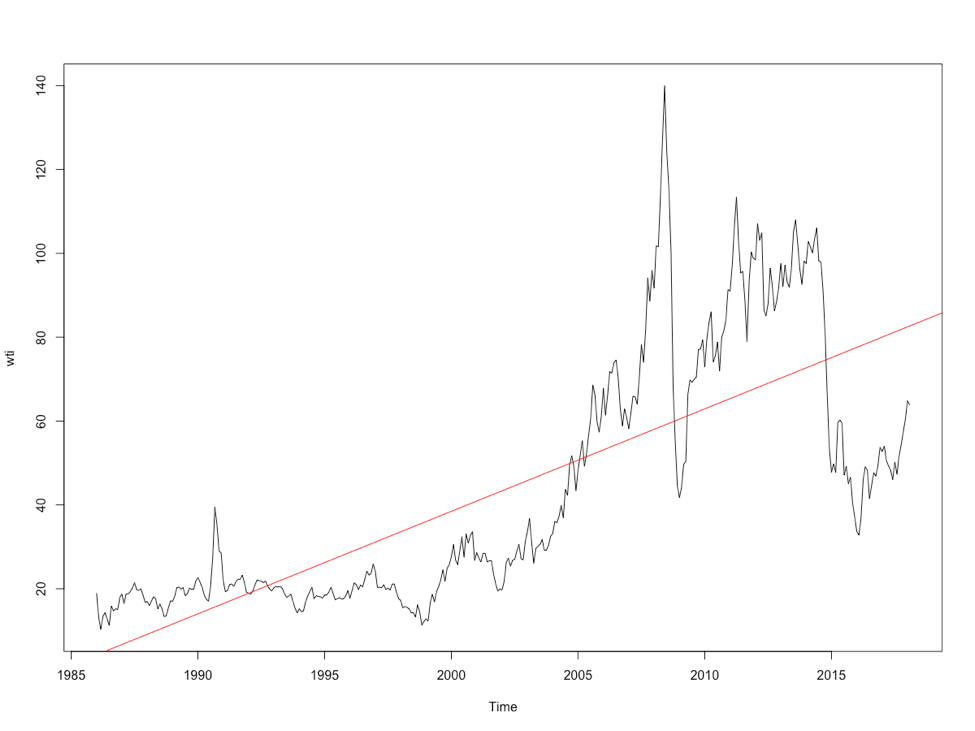
\includegraphics[width=5in]{regresionTiempoWTI}\\
	\caption{Descomposición STL Precio Internacional del Café (Fuente Propia)}
\end{figure}

\subsection{Modelo Predictivo Ensamblado}
El modelo predictivo ensamblado es el resultado del entrenamiento de un modelo predictivo de regresión lineal y un modelo ARIMA. Ambos modelos se combinan y se entrenan con la variable de valor real en común para ambos \cite{viswanathan}.

\begin{lstlisting}[language=R]
# Pseudo-codigo R simplificado
# Funcion de modelo ensamblado

# Cargar Data Frame con informacion de series de tiempo
library(caret)
set.seed(7556014)
data(featuresTRM)
data(TRM)
adData = data.frame(TRM, featuresTRM)
inTrain = createDataPartition(adData$TRM, p = 3/4)[[1]]
training = adData[ inTrain,]
testing = adData[-inTrain,]

set.seed(7556014)

modelo1 <- train(TRM ~ ., method = "glm", data = training)
modelo2 <- train(TRM ~ ., method = "ARIMA", data = training)

# Vectores de valores de prediccion de cada modelo
predVec1 <- predict(modelo1, testing)
predVec2 <- predict(modelo2, testing)

# Construccion de matriz de datos ensamblados (variable dependiente y predictor)
predDF <- data.frame(TRM = testing$TRM, predVec1, predVec2)

# Modelo combinado (fit)
combModelFit <- train(TRM ~ ., method = "glm", data = predDF)
finalPred <- predict(combModelFit, predDF)
\end{lstlisting}

\section{Diseño de muestreo}

Inicialmente, podemos calcular el tamaño de la muestra necesaria para nuestro estudio con la fórmula \cite{mendehall}:

\begin{equation}
   n =  (N* z^2*p*q)/(E^2*(N-1)+ z^2*p*q)
\end{equation}

El tamaño total de todas las cotizaciones de la TRM o del precio internacional del petróleo WTI es un número finito. Los mercados funcionan de lunes a viernes, por lo general las cincuenta y dos semanas del año. Para el uso común de la tasa de cambio, esta cifra se usa todos los días, por ejemplo cuando un consumidor usa una tarjeta de crédito y el banco debe referir al valor de la TRM aunque no sea día de operaciones bursátiles. Por lo que el número total de posibles cotizaciones oficiales en un año dado cualesquiera se determinan como:

\begin{equation}
    N_{regresor} = 365
\end{equation}

La fórmula es muy simple y equivale a sustituir cualquier variable regresor (por ejemplo, el valor del petróleo WTI) por los números reales de días del año.

\begin{equation}
    N_{wti} = 365
\end{equation}

Ende, existen 365 posibles valores de la cotización del petróleo WTI en un año cualesquiera. Dado que el modelo de predicción de aprendizaje automatizado utiliza datos del año 2010 al 2017 inclusive, podemos ampliar el universo dentro del período de estudio con la siguiente formula:
\begin{equation}
    n_{regresor} = 365 * 8 = 2920
\end{equation}

Nuestro universo por regresor equivale a dos mil novecientos veinte puntos de datos. Para un estudio con un nivel de confianza del 99\% y un error de estimación del 5\% calculamos el número de la muestra como una proporción, donde:

\begin{eqnarray*}
  N &=& 2,080 \text{ puntos de datos} \\
  p &=& 0.5 \\
  q &=& 0.5 \text{ o (1 – p)} \\
  z &=& 99\% \text{ o 2.575} \\
  e &=& 5\% \text{ o 0.05} \\
\end{eqnarray*}

Utilizamos el lenguaje R para resolver el cálculo:

\begin{lstlisting}[language=R]
N <- 2080
p <- 0.5
q <- 1 - p
z <- 2.575
E <- 0.05

muestra <- (N * z^2 * p * q) / ((N - 1) * E^2 + z^2 * p * q)
muestra
[1] 502.9681
\end{lstlisting}

El tamaño de la muestra es 503 puntos de datos por regresor a utilizar. Sin embargo, dado que los usos de técnicas de Ciencia de Datos nos permiten acceder a la biblioteca Quandl de forma de recolectar el universo entero de datos, utilizaremos los 2,920 puntos de datos para cada regresor, trabajando de esta forma con el universo entero y no la muestra. Este es un buen ejemplo del uso de Big Data \cite{pengMatsui} que no solo aplica a muestras grandes de universos extensos, sino al total de la data de un universo pequeño.

\subsubsection{Reglas de Imputación de Datos}
Es común que las bases de datos retornen series de datos incompletas para los días feriados o días sin cambio en la cotización del bien. Para determinar el valor de cualquier día incompleto, la investigación resolvió el método de imputación como la última cotización válida para el regresor.

\subsection{Observaciones Adicionales Sobre el Uso de Muestras dentro de Diseños de Investigación con Regresión Lineal}
No todos los autores están de acuerdo con el uso de la fórmula tradicional para el cálculo del número de muestras en un estudio de regresión lineal. William Dupont y Walton Plummer han discutido el uso de técnicas alternativas cuando los estudios (sobre todo los estudios clínicos) utilizan regresiones lineales multivariable \cite{dupontPlummer}. Dichas técnicas se apoyan en la identificación de diferentes pendientes en los análisis de regresión versus el uso de coeficientes (argumentando que es más fácil comparar visualmente pendientes versus coeficientes) y el manejo del poder estadístico $1 – \beta$. Sobre este último los autores manifiestan ajustar los niveles de poder para verificar en que momento del cambio se detecta diferencias de la pendiente de una hipótesis contra su hipótesis alternativa dentro de una muestra de n pacientes.

Al momento de preparar el diseño del estudio, las herramientas de medición y la muestra, el doctorando ha decidido no profundizar más en métodos menos tradicionales de cálculo de muestras en estudios de regresión lineal, dado que en el caso específico se utilizará la totalidad del universo, haciendo el cálculo de muestra innecesario.
